\documentclass[11pt,letterpaper]{article}

\usepackage[margin=0.78in,headheight=15pt]{geometry}
\usepackage[T1]{fontenc}
\usepackage[utf8]{inputenc}
\usepackage{amsmath}
\usepackage{newpxtext}
\usepackage{newpxmath}
\usepackage[scaled=0.90]{inconsolata}
\usepackage{microtype}
\DisableLigatures{encoding = *, family = tt*}
\usepackage{booktabs}
\usepackage{tabularx}
\usepackage{caption}
\usepackage{enumitem}
\usepackage{float}
\usepackage{graphicx}
\usepackage{needspace}
\usepackage[table]{xcolor}
\usepackage[most]{tcolorbox}
\usepackage{parskip}
\usepackage{titlesec}
\usepackage{upquote}
\usepackage{fancyhdr}

\definecolor{primary}{HTML}{0F4C5C}
\definecolor{accent}{HTML}{137C8B}
\definecolor{bannerbg}{HTML}{F0F7F9}
\definecolor{calloutbg}{HTML}{F4F9FA}
\definecolor{codebg}{HTML}{F1F5F9}
\definecolor{codeborder}{HTML}{CBD5E1}
\definecolor{figborder}{HTML}{DCE4EC}
\definecolor{rowalt}{HTML}{F8FAFC}
\definecolor{muted}{HTML}{475569}
\definecolor{rulecol}{HTML}{CBD5E1}

\usepackage[colorlinks=true,urlcolor=accent,linkcolor=accent]{hyperref}
\pdfstringdefDisableCommands{\def\code#1{#1}}

\captionsetup{font=small,labelfont={bf,color=primary},skip=4pt}
\graphicspath{{figures/}{docs/latex/figures/}}

\titleformat{\section}
  {\large\bfseries\color{primary}}
  {\thesection.}
  {0.5em}
  {}
  [\vspace{-0.45em}\color{accent!40}\rule{\linewidth}{0.6pt}]
\titleformat{\subsection}
  {\normalsize\bfseries\color{primary}}
  {\thesubsection}
  {0.5em}
  {}

\titlespacing*{\section}{0pt}{0.75em}{0.35em}
\titlespacing*{\subsection}{0pt}{0.55em}{0.2em}

\setlist[itemize]{leftmargin=1.4em,itemsep=0.18em,topsep=0.15em}
\setlist[enumerate]{leftmargin=1.6em,itemsep=0.22em,topsep=0.18em}

\pagestyle{fancy}
\fancyhf{}
\lhead{\small\color{muted}CSI 5550 -- Visual Computing}
\rhead{\small\color{muted}From Pixels to Predictions}
\cfoot{\small\color{muted}\thepage}
\renewcommand{\headrulewidth}{0.4pt}
\renewcommand{\headrule}{\color{rulecol}\hrule width\headwidth height\headrulewidth \vskip-\headrulewidth}

\newcommand{\code}[1]{\texttt{\textcolor{primary}{#1}}}
\newcommand{\codelink}[2]{\href{#1}{\texttt{#2}}}

\newtcolorbox{codeblock}{
  enhanced,
  colback=codebg,
  colframe=codeborder,
  borderline west={2.5pt}{0pt}{accent},
  arc=2.5pt,
  boxrule=0.4pt,
  left=8pt,
  right=8pt,
  top=5pt,
  bottom=5pt,
  fontupper=\small\ttfamily,
  before skip=0.3em,
  after skip=0.45em,
}

\newtcolorbox{calloutbox}[1][]{
  enhanced,
  colback=calloutbg,
  colframe=calloutbg,
  borderline west={2.5pt}{0pt}{accent},
  arc=2pt,
  boxrule=0pt,
  left=8pt,
  right=8pt,
  top=5pt,
  bottom=5pt,
  before skip=0.35em,
  after skip=0.45em,
  #1
}

\newcommand{\evalbadge}[1]{%
  \par\vspace{0.15em}\noindent%
  \tcbox[
    on line,
    boxsep=2pt,
    left=6pt,
    right=6pt,
    top=2pt,
    bottom=2pt,
    colback=bannerbg,
    colframe=accent!35,
    boxrule=0.4pt,
    arc=2pt
  ]{\small #1}%
  \par\vspace{0.2em}%
}

\newcommand{\figcard}[1]{%
  \begin{tcolorbox}[
    enhanced,
    colback=white,
    colframe=figborder,
    boxrule=0.5pt,
    arc=3pt,
    left=5pt,
    right=5pt,
    top=5pt,
    bottom=5pt,
    before skip=0.15em,
    after skip=0.25em
  ]
    \centering
    #1
  \end{tcolorbox}%
}

\begin{document}

\begin{tcolorbox}[
  enhanced,
  colback=bannerbg,
  colframe=accent!35,
  borderline west={4pt}{0pt}{primary},
  arc=3pt,
  boxrule=0.5pt,
  left=12pt,
  right=12pt,
  top=8pt,
  bottom=8pt,
  before skip=0pt,
  after skip=0.45em
]
  {\small\bfseries\color{accent} CSI 5550 \enspace\textperiodcentered\enspace VISUAL COMPUTING \enspace\textperiodcentered\enspace LABORATORY ASSIGNMENT}\\[0.25em]
  {\fontsize{19}{22}\selectfont\bfseries\color{primary} From Pixels to Predictions}\\[0.15em]
  {\normalsize\color{muted} Measuring CNN Sensitivity to Classical Image Processing Operators}\\[0.35em]
  {\color{accent!30}\hrule height 0.5pt}\vspace{0.35em}
  {\renewcommand{\arraystretch}{1.08}%
  \begin{tabular*}{\linewidth}{@{\extracolsep{\fill}}lll@{}}
    {\scriptsize\bfseries\color{accent} CLASSIFIER} &
    {\scriptsize\bfseries\color{accent} DATASET} &
    {\scriptsize\bfseries\color{accent} SUBMISSION} \\
    {\footnotesize ResNet-18 (\code{IMAGENET1K\_V1})} &
    {\footnotesize 200 Imagenette Images} &
    {\footnotesize\code{visual\_computing\_lab.ipynb}}
  \end{tabular*}}
\end{tcolorbox}

\section{Overview and Experimental Setup}

In this laboratory, you will implement six classical image processing operators---spatial sampling, intensity quantization, affine rotation, histogram equalization (with a histogram counter helper), Gaussian smoothing, and Laplacian sharpening---from first principles in PyTorch. You will then evaluate \textbf{your own implementations} as front-end transformations before a pre-trained convolutional neural network to measure how signal resolution, geometry, contrast, blur, and high-frequency emphasis change predictions and confidence.

\subsection{Model and Dataset}
\begin{itemize}
  \item \textbf{Classifier:} ResNet-18 loaded with TorchVision's published \code{IMAGENET1K\_V1} weights. No training or fine-tuning is performed. Model outputs are restricted to the 10 Imagenette categories (\textit{tench, English springer, cassette player, chain saw, church, French horn, garbage truck, gas pump, golf ball, parachute}), and confidence is the conditional 10-class softmax probability (the model's raw scores converted into probabilities that sum to $1$ across those 10 classes). Because Imagenette is derived from ImageNet, this lab is a controlled sensitivity study rather than an independent generalization benchmark.
  \item \textbf{Dataset:} One fixed, class-balanced subset of 200 images (20 per class) from \code{imagenette2-320/val}, recorded in \code{data/lab\_subset.json}. Each image is provided to your functions as a $224 \times 224$ RGB tensor with floating-point pixel intensities in $[0, 1]$, and every condition is evaluated on the exact same 200 images.
\end{itemize}

\subsection{Quick Start}
This project uses \code{uv} for environment and package management. If \code{uv} is not installed yet, follow \href{https://docs.astral.sh/uv/getting-started/installation/}{the official \code{uv} installation guide} or run the standalone installer for your platform:
\begin{itemize}[itemsep=0.12em,topsep=0.08em,parsep=0pt]
  \item \textbf{macOS / Linux:} {\small\code{curl -LsSf https://astral.sh/uv/install.sh | sh}}
  \item \textbf{Windows (PowerShell):}\\[-0.15em]
    {\small\code{powershell -ExecutionPolicy ByPass -c "irm https://astral.sh/uv/install.ps1 | iex"}}
\end{itemize}
After installing \code{uv} (restart your terminal if needed), run these commands from the project root directory to synchronize the environment, cache the dataset and weights once, and open JupyterLab (select the project's \code{.venv} kernel):
\begin{codeblock}
uv sync --locked\\
uv run --locked cnn-signal-sensitivity prepare\\
uv run --locked jupyter lab
\end{codeblock}
Open \code{notebooks/visual\_computing\_lab.ipynb}. Each exercise is followed immediately by a visual demonstration and a public unit check in \code{cnn\_signal\_sensitivity.checks}. The six operators are independent: you can implement and test them in any order, skip a function if you get stuck, and come back to it later (note that \code{histogram\_equalize} in D2 may optionally call \code{image\_histogram} from D1, and the full comparative evaluation in Section 4 runs once all operators are completed).

\newpage
\section{General Operator Contract}

Unless noted otherwise, every function you implement must satisfy:
\begin{enumerate}
  \item \textbf{Input/output tensor contract:} Accept a batch \code{images} of shape $(B, 3, H, W)$ with floating-point RGB values in $[0, 1]$. Return a tensor with the exact same shape, \code{dtype}, and \code{device} (except \code{image\_histogram}, which returns \code{torch.long} counts of shape $(B, 256)$ on the input device).
  \item \textbf{Immutability:} Never modify \code{images} in place (do not overwrite the input tensor directly); return a new tensor or a copy (\code{images.clone()}) when returning an unchanged image.
  \item \textbf{Vectorized PyTorch:} Use vectorized PyTorch tensor operations (computing across whole tensors at once rather than nested Python \code{for} loops over individual pixels; iterating over the batch dimension $B$ when needed for per-image operations is fine).
  \item \textbf{Parameter validation:} Raise \code{ValueError} for invalid arguments (e.g., non-positive or non-integer sampling factors, bit depths outside $[1, 8]$, non-finite angles, negative or non-finite filter strengths, or Gaussian kernel radius $\ge \min(H, W)$).
  \item \textbf{Public checks:} Each exercise has its own unit check cell so you can verify that operator independently as soon as you write it. Passing the check confirms the core contract, though you should still consider edge cases such as non-square inputs, multi-image batches, and constant images.
\end{enumerate}

\section{Operator Specifications (Seven Exercises)}

\subsection{A. Image Sampling and Nearest-Neighbor Interpolation (\code{sample\_image})}
Subsample spatially (reduce resolution by keeping only a subset of pixels) by taking every $s$-th row and column (starting at index $0$) for positive integer \code{factor} $s \ge 1$. Reconstruct the original $(H, W)$ spatial dimensions via \textbf{nearest-neighbor interpolation} (filling each output pixel with the value of the closest retained sample) by repeating each retained sample $s$ times along height and width, then cropping any excess rows or columns back to $(H, W)$. When $s = 1$, reproduce the input unchanged.

\begin{calloutbox}
  \small\textbf{Design note:} \textbf{Anti-aliasing} (pre-smoothing an image before subsampling to prevent fine, high-frequency patterns from folding into false jagged or stair-step artifacts known as \textbf{aliasing}) is intentionally omitted here so you can observe aliasing and high-frequency detail loss directly.
\end{calloutbox}

\evalbadge{\textbf{Evaluated settings:} $s \in \{1, 2, 4, 8, 16\}$}

\begin{figure}[H]
  \figcard{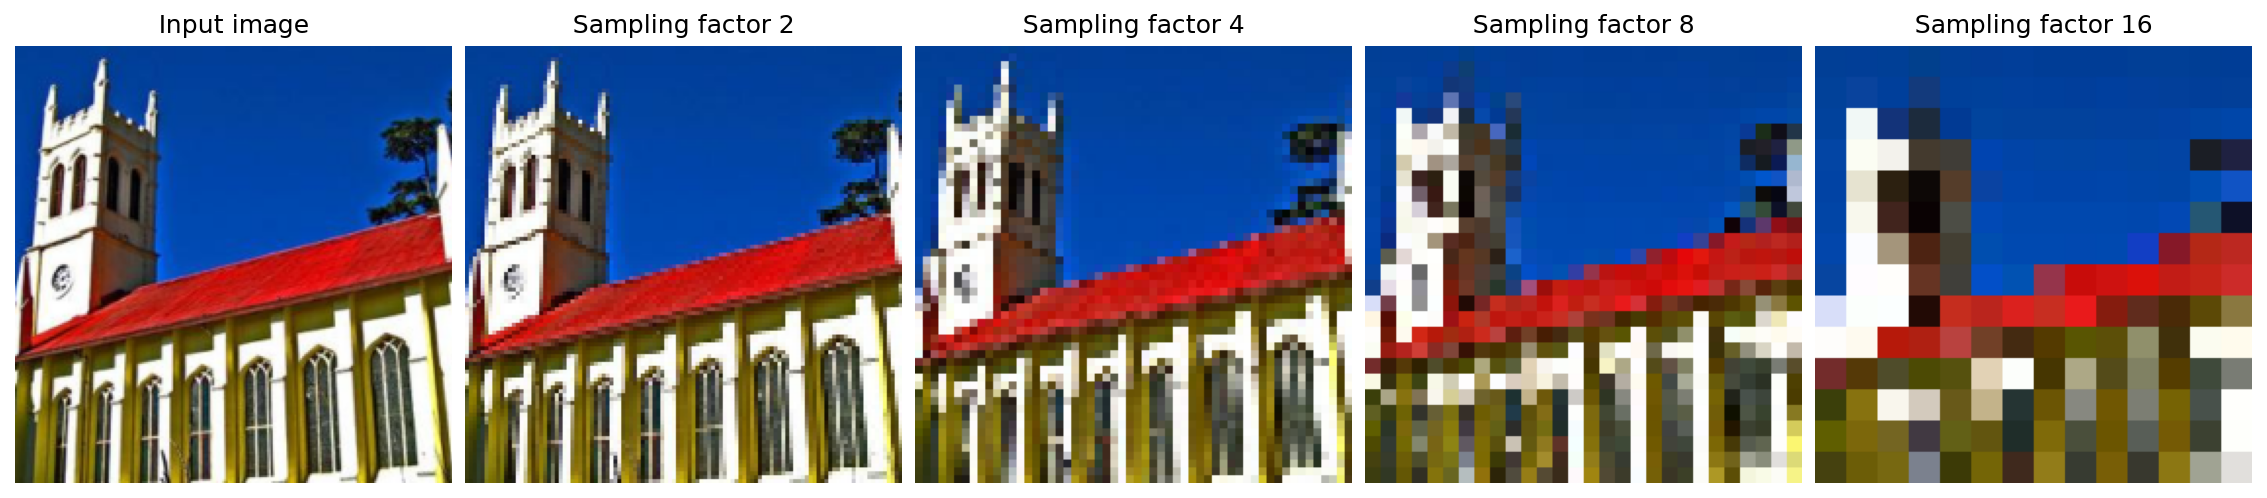
\includegraphics[width=\linewidth]{demo_sample_image.png}}
  \caption{Input image and expected \code{sample\_image} outputs for factors $s \in \{2, 4, 8, 16\}$.}
\end{figure}

\subsection{B. Intensity Quantization (\code{quantize})}
Reduce per-channel intensity precision (\textbf{quantization}: mapping continuous or fine brightness values to a smaller finite set of discrete levels) to $2^b$ uniformly spaced levels in $[0, 1]$ for integer \textbf{bit depth} $b \in \{1, 2, \dots, 8\}$ (where $b$ bits per color channel represent $2^b$ possible intensity levels):
\[
  Q_b(x) = \frac{\mathrm{round}\!\left((2^b - 1)\,x\right)}{2^b - 1}.
\]
This endpoint-preserving formula keeps $0$ and $1$ exact and preserves standard 8-bit image samples when $b = 8$.

\evalbadge{\textbf{Evaluated settings:} $b \in \{8, 6, 4, 3, 2, 1\}$ bits/channel}

\begin{figure}[H]
  \figcard{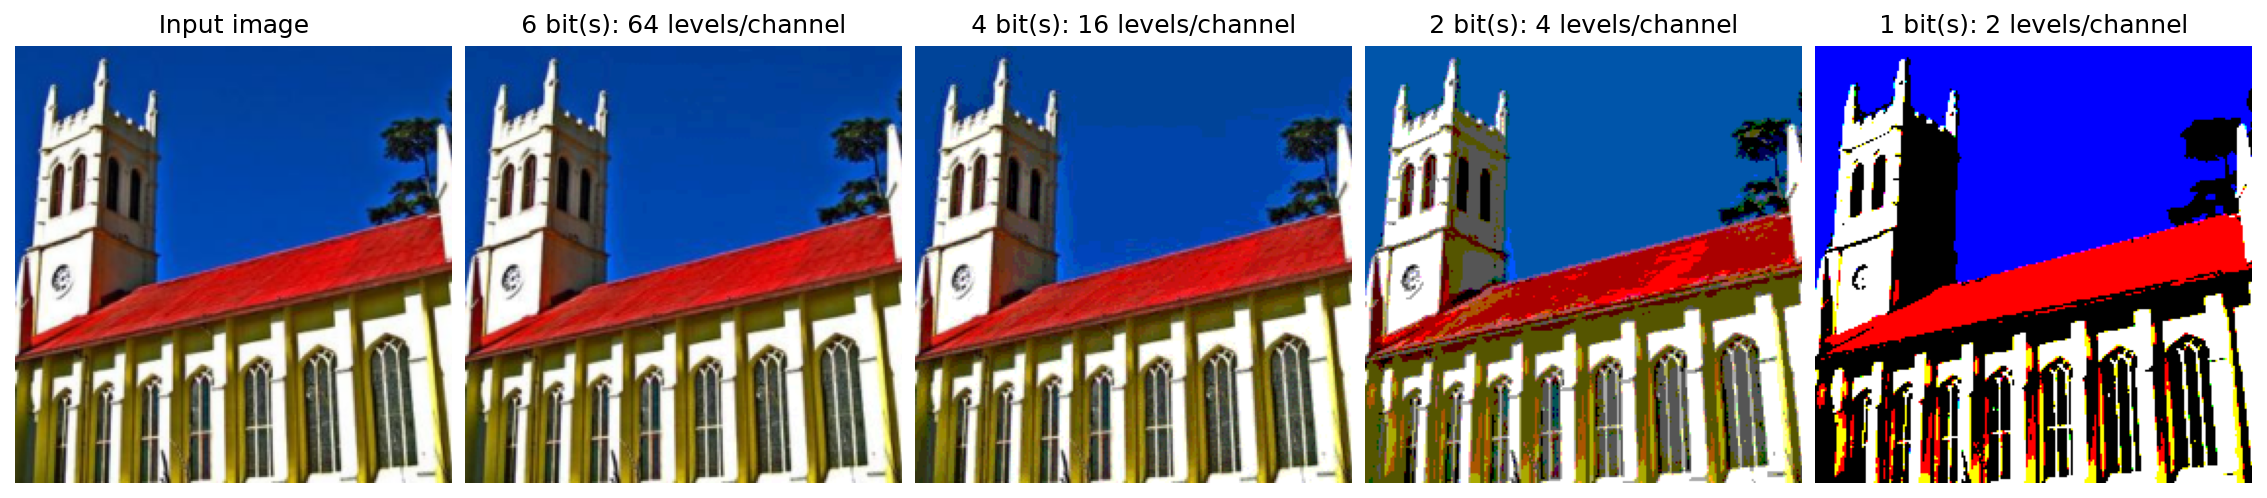
\includegraphics[width=\linewidth]{demo_quantize.png}}
  \caption{Input image and expected \code{quantize} outputs for $b \in \{6, 4, 2, 1\}$ bits per channel.}
\end{figure}

\subsection{C. Affine Geometric Transformation (\code{affine\_rotation})}
Rotate every image in the batch counterclockwise by \code{angle} $\theta$ (in degrees) about its center using \textbf{inverse coordinate mapping} (for each pixel location in the \emph{output} image, computing where it came from in the \emph{input} image so every output pixel receives a value without gaps) and \textbf{bilinear interpolation} (computing a distance-weighted average of the four surrounding input pixels when a mapped coordinate lands between integer grid locations), keeping the $(H, W)$ canvas fixed. Outside regions beyond the source image bounds $[0, W-1] \times [0, H-1]$ must be filled with neutral gray ($0.5$) (treating out-of-bounds source samples as $0.5$ during interpolation), with final outputs \textbf{clamped} (restricted so values below $0$ become $0$ and values above $1$ become $1$) to $[0, 1]$. When $\theta = 0$, return a clone of \code{images}. Do not replace this exercise with a ready-made rotation helper.

\begin{calloutbox}
  \small\textbf{Coordinate conventions:} Let $x \in \{0, \dots, W-1\}$ increase rightward and $y \in \{0, \dots, H-1\}$ increase downward, with image center $(c_x, c_y) = \bigl((W-1)/2,\,(H-1)/2\bigr)$. For each centered output coordinate $(\hat{x}, \hat{y}) = (x - c_x,\, y - c_y)$, compute the source location in pixel coordinates:
  \[
    x_s = \hat{x}\cos\theta - \hat{y}\sin\theta + c_x, \qquad
    y_s = \hat{x}\sin\theta + \hat{y}\cos\theta + c_y.
  \]
\end{calloutbox}

\evalbadge{\textbf{Evaluated settings:} $\theta \in \{-45^\circ, -30^\circ, -15^\circ, 0^\circ, 15^\circ, 30^\circ, 45^\circ\}$}

\begin{figure}[H]
  \figcard{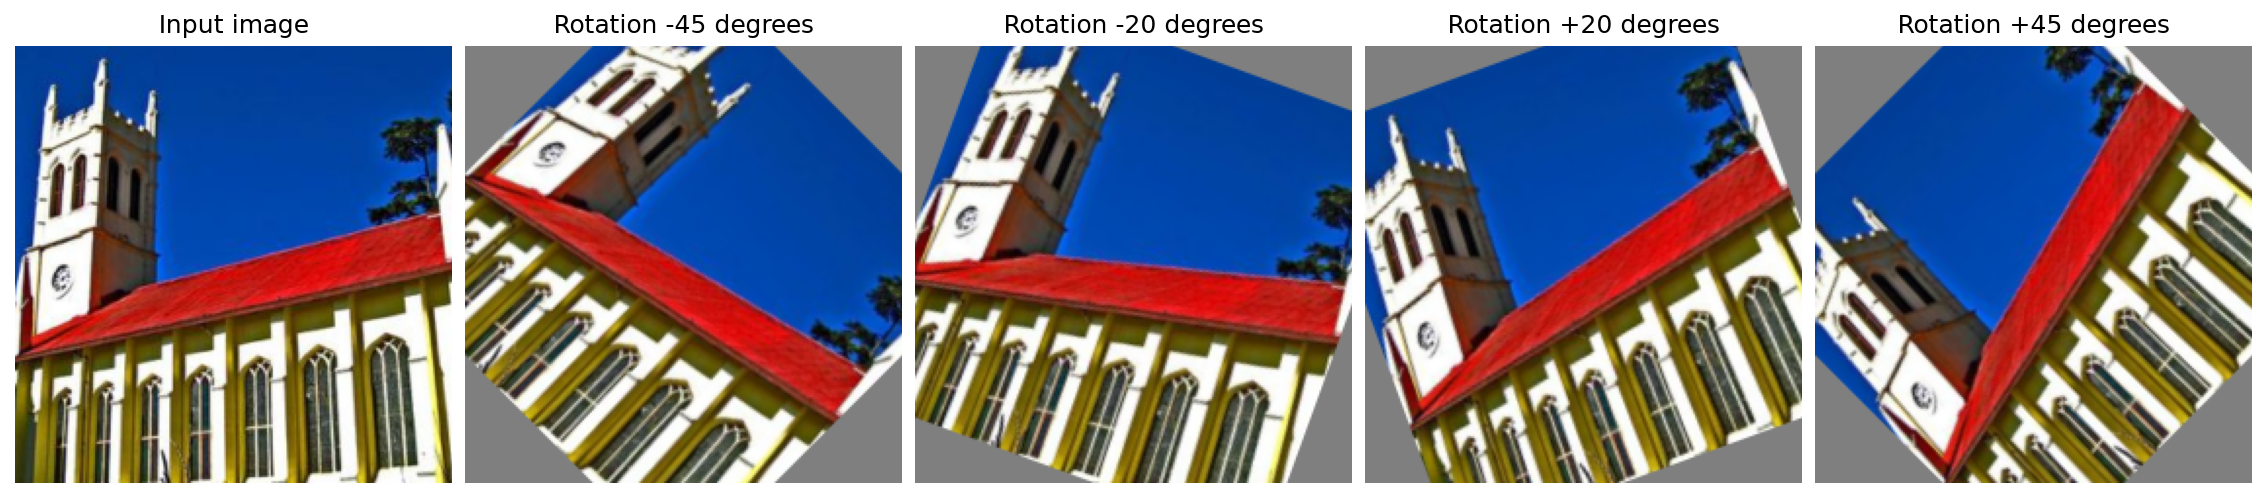
\includegraphics[width=\linewidth]{demo_affine_rotation.png}}
  \caption{Input image and expected \code{affine\_rotation} outputs for $\theta \in \{-45^\circ, -20^\circ, +20^\circ, +45^\circ\}$.}
\end{figure}

\subsection{D1. Image Histogram (\code{image\_histogram})}
Compute the arithmetic-mean grayscale intensity $I = \frac{1}{3}(R + G + B)$ for each pixel, and assign bin indices $k = \mathrm{round}(255\,I) \in \{0, 1, \dots, 255\}$. Return a \code{torch.long} tensor of shape $(B, 256)$ on the input device where row $i$ contains the pixel counts for image $i$ (each row sums to $H \times W$). You will use this function to plot the input and equalized histograms on shared axes.

\begin{figure}[H]
  \figcard{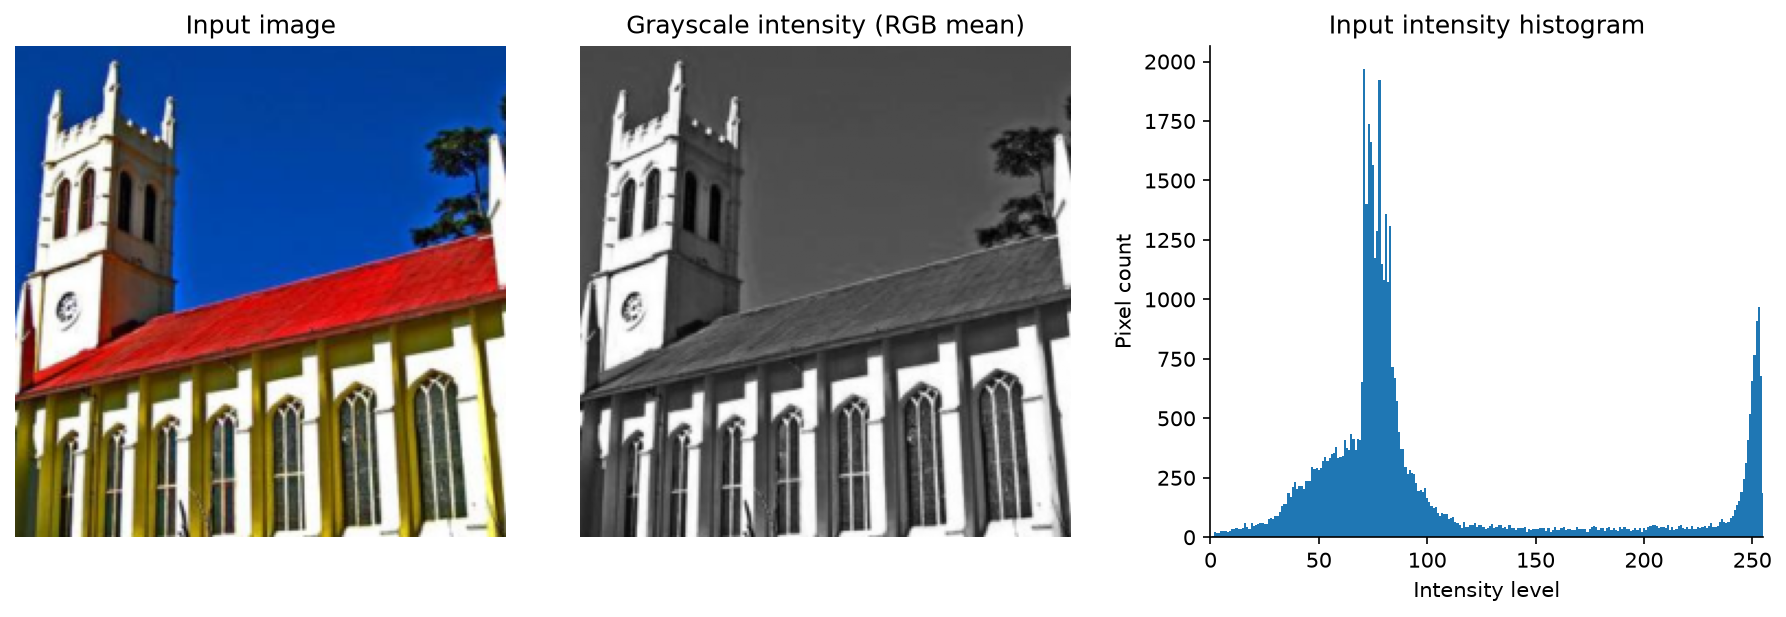
\includegraphics[width=0.92\linewidth]{demo_image_histogram.png}}
  \caption{Input RGB image, mean grayscale intensity $I = (R+G+B)/3$, and expected 256-bin histogram counts from \code{image\_histogram}.}
\end{figure}

\subsection{D2. Histogram Equalization (\code{histogram\_equalize})}
Redistribute grayscale intensities independently for each image using its 256-bin histogram (you may call \code{image\_histogram}) and cumulative distribution $\mathrm{CDF}(k) = \sum_{j=0}^{k} h(j)$ (the running total of pixels with bin index $\le k$). Let $\mathrm{CDF}_{\min}$ be the cumulative count of the first occupied bin (smallest $k$ with $h(k) > 0$). If all pixels occupy a single bin ($\mathrm{CDF}(255) - \mathrm{CDF}_{\min} = 0$), preserve the constant grayscale intensity unchanged; otherwise map each pixel's bin $k$ through
\[
  T(k) = \frac{\mathrm{CDF}(k) - \mathrm{CDF}_{\min}}{HW - \mathrm{CDF}_{\min}}
  \;=\; \frac{\widetilde{\mathrm{CDF}}(k) - \widetilde{\mathrm{CDF}}_{\min}}{1 - \widetilde{\mathrm{CDF}}_{\min}},
\]
where $\widetilde{\mathrm{CDF}} = \mathrm{CDF}/(HW)$ is the normalized CDF, clamped (restricted) to $[0, 1]$. Replicate the equalized intensity across all three RGB channels so the output shape is $(B, 3, H, W)$.

\begin{calloutbox}
  \small\textbf{Experimental control:} Because equalization removes color as well as changing contrast, Section 4 evaluates both \code{grayscale} (arithmetic RGB mean replicated to 3 channels) and \code{equalized} to isolate contrast redistribution from color removal.
\end{calloutbox}

\begin{figure}[H]
  \figcard{%
    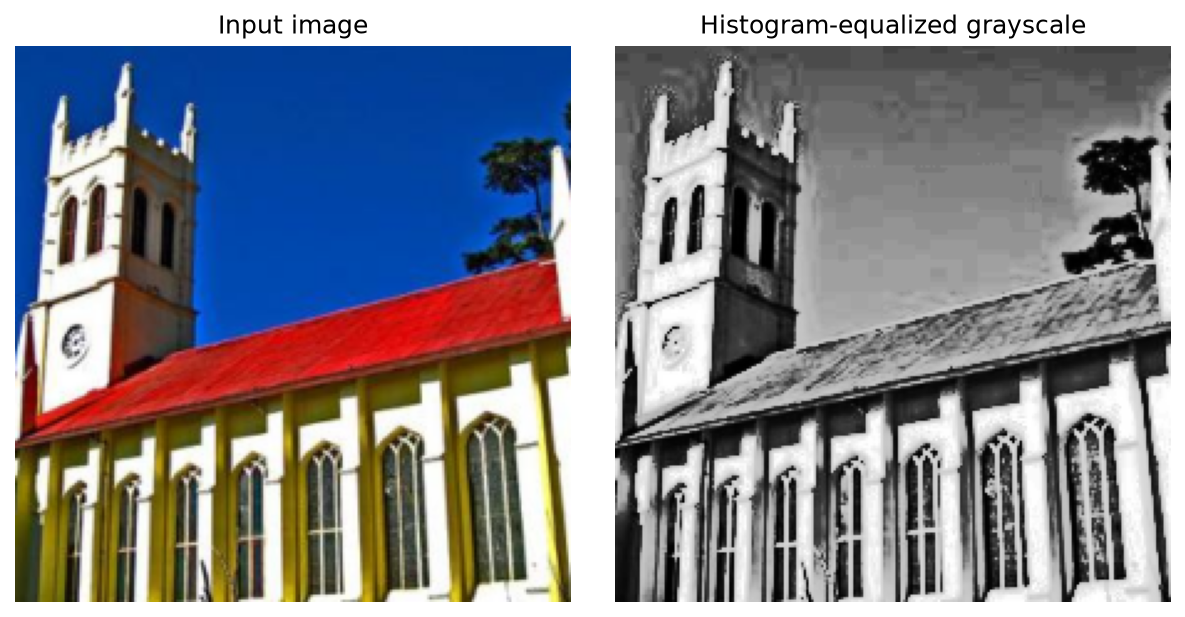
\includegraphics[width=0.72\linewidth]{demo_histogram_equalize.png}\\[6pt]
    {\color{figborder}\rule{0.92\linewidth}{0.5pt}}\\[6pt]
    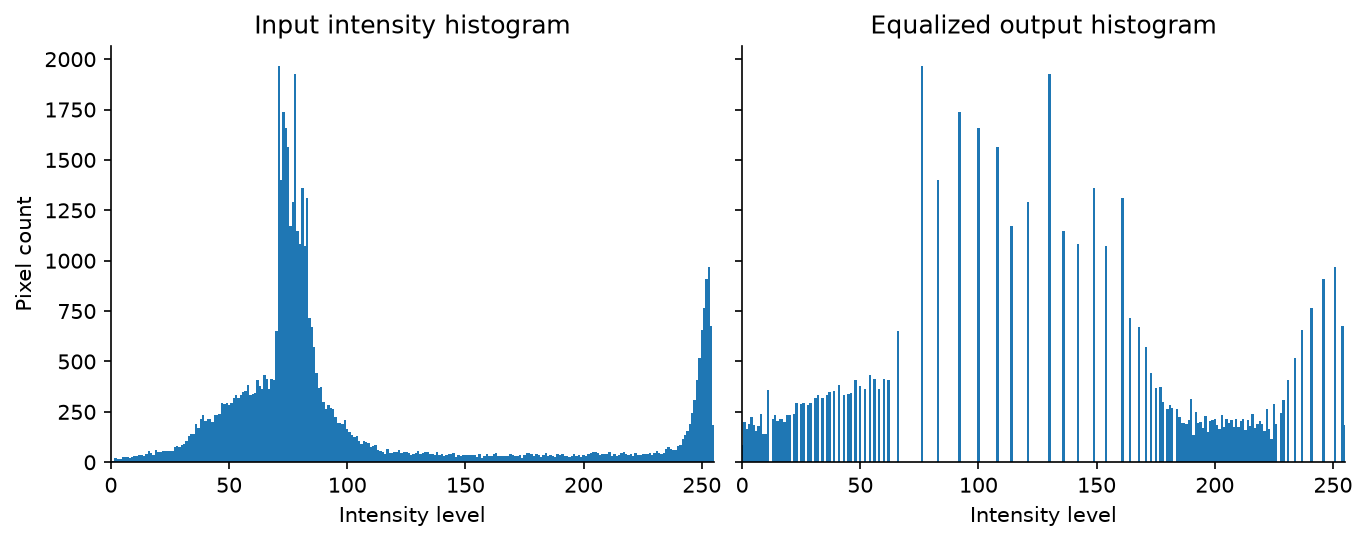
\includegraphics[width=0.88\linewidth]{histogram_comparison.png}%
  }
  \caption{Top: input image and expected \code{histogram\_equalize} output. Bottom: corresponding 256-bin intensity histograms.}
\end{figure}

\subsection{E. Gaussian Smoothing (\code{gaussian\_smooth})}
Attenuate rapid pixel-to-pixel intensity variations (\textbf{high-frequency detail}) using a circularly symmetric (\textbf{isotropic}) 2-D Gaussian kernel with standard deviation \code{sigma} $\sigma \ge 0$ (in pixels). When $\sigma = 0$, return a clone of \code{images}. Otherwise set kernel radius $r = \lceil 3\sigma \rceil$ (raising \code{ValueError} if $r \ge \min(H, W)$), evaluate
\[
  K(x, y) = e^{-\frac{x^2 + y^2}{2\sigma^2}}, \quad x, y \in \{-r, \dots, r\},
\]
and normalize so $\sum_{x, y} K(x, y) = 1$. Pad borders by $r$ pixels using \textbf{reflection padding} (extending the image boundary by mirroring interior pixel values across the edge so the filter window has valid neighbors at border pixels without introducing artificial dark or bright seams), filter each RGB channel independently, and \textbf{clamp} (restrict) outputs to $[0, 1]$.

\evalbadge{\textbf{Evaluated settings:} $\sigma \in \{0, 0.5, 1, 2, 4\}$ pixels}

\begin{figure}[H]
  \figcard{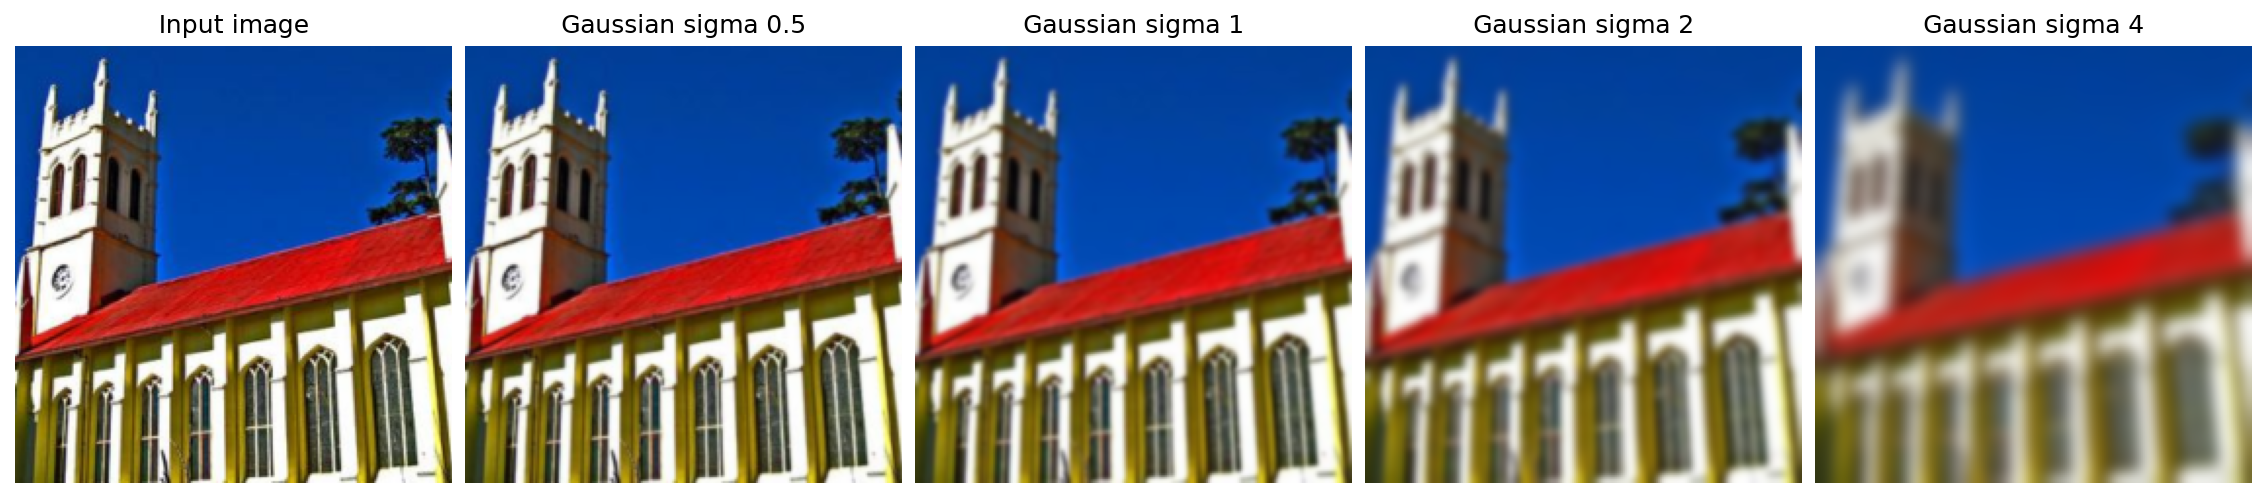
\includegraphics[width=\linewidth]{demo_gaussian_smooth.png}}
  \caption{Input image and expected \code{gaussian\_smooth} outputs for $\sigma \in \{0.5, 1, 2, 4\}$ pixels.}
\end{figure}

\subsection{F. Laplacian Sharpening (\code{laplacian\_sharpen})}
Emphasize rapid intensity transitions using the discrete four-neighbor Laplacian kernel:
\[
  L = \begin{bmatrix} 0 & 1 & 0 \\ 1 & -4 & 1 \\ 0 & 1 & 0 \end{bmatrix}.
\]
For nonnegative sharpening strength \code{amount} $a \ge 0$ ($a = 0$ returns a clone), pad \code{images} by $1$ pixel on all sides using \textbf{reflection padding} (mirroring interior pixels across the border), filter each RGB channel independently to obtain the \textbf{signed} response $\nabla^2 f$ (retaining both positive and negative filter values rather than taking absolute values), and compute
\[
  g = \mathrm{clamp}\!\left(f - a\,\nabla^2 f,\, 0,\, 1\right),
\]
where $\mathrm{clamp}(v, 0, 1)$ restricts values below $0$ to $0$ and values above $1$ to $1$ (also called \emph{clipping}). Keep the signed response before subtraction (do not take $|\nabla^2 f|$) and clip only after subtracting from the original image.

\evalbadge{\textbf{Evaluated settings:} $a \in \{0, 0.25, 0.5, 1, 2\}$}

\begin{figure}[H]
  \figcard{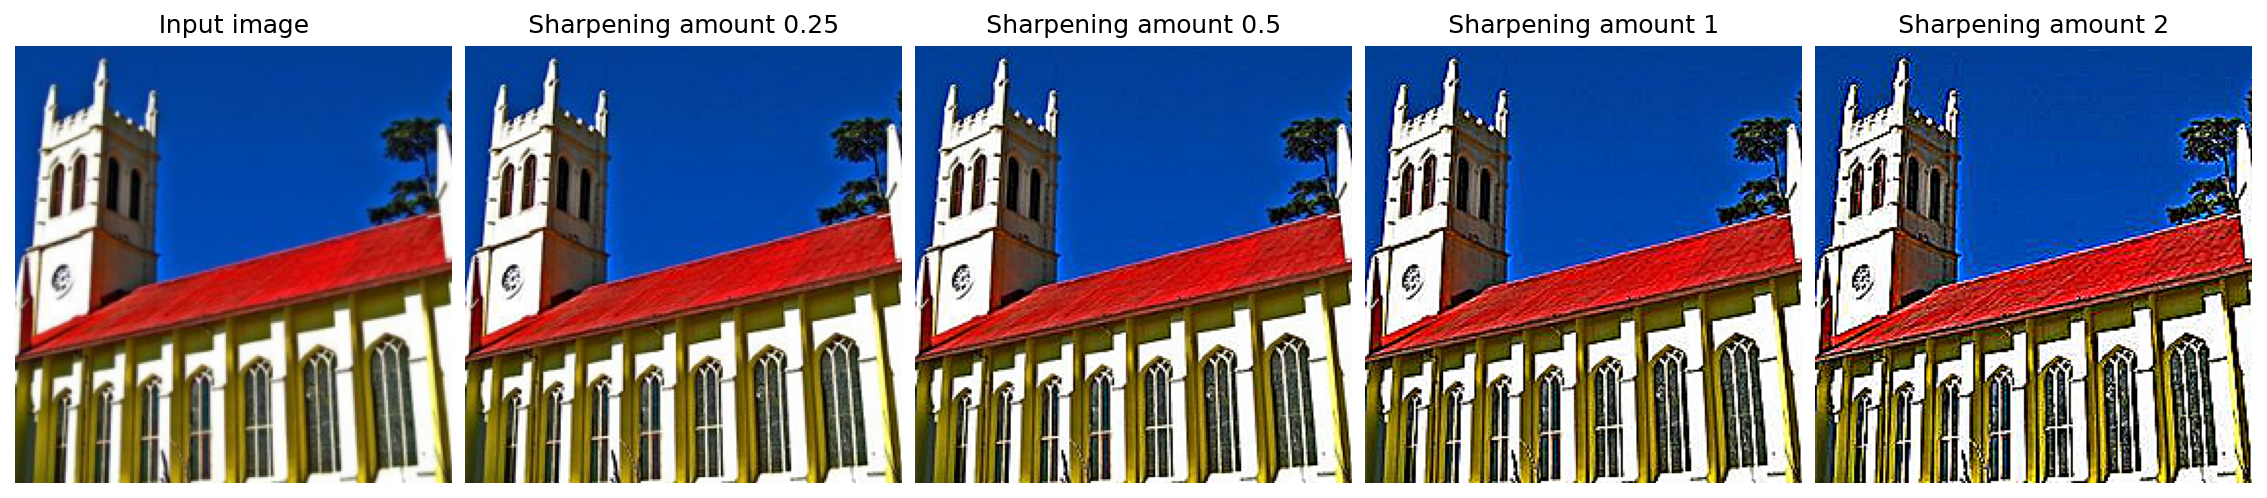
\includegraphics[width=\linewidth]{demo_laplacian_sharpen.png}}
  \caption{Input image and expected \code{laplacian\_sharpen} outputs for sharpening amounts $a \in \{0.25, 0.5, 1, 2\}$.}
\end{figure}

\needspace{11\baselineskip}
\subsection{Helpful PyTorch Functions (Optional)}
\begin{calloutbox}[breakable]
You are encouraged to explore any vectorized PyTorch design that satisfies the specifications above. The functions below are optional building blocks you can check out---click any name to open its official PyTorch documentation, or use another approach if you prefer:
\begin{itemize}\raggedright
  \item \textbf{Sampling \& shape manipulation:}
    \codelink{https://docs.pytorch.org/docs/stable/generated/torch.repeat_interleave.html}{torch.repeat\_interleave},
    \codelink{https://docs.pytorch.org/docs/stable/generated/torch.Tensor.repeat.html}{torch.Tensor.repeat},
    \codelink{https://docs.pytorch.org/docs/stable/generated/torch.Tensor.expand.html}{torch.Tensor.expand}.
  \item \textbf{Rounding \& value bounds:}
    \codelink{https://docs.pytorch.org/docs/stable/generated/torch.round.html}{torch.round},
    \codelink{https://docs.pytorch.org/docs/stable/generated/torch.clamp.html}{torch.clamp},
    \codelink{https://docs.pytorch.org/docs/stable/generated/torch.floor.html}{torch.floor},
    \codelink{https://docs.pytorch.org/docs/stable/generated/torch.ceil.html}{torch.ceil}.
  \item \textbf{Coordinate grids \& warping:}
    \codelink{https://docs.pytorch.org/docs/stable/generated/torch.arange.html}{torch.arange},
    \codelink{https://docs.pytorch.org/docs/stable/generated/torch.meshgrid.html}{torch.meshgrid},
    \codelink{https://docs.pytorch.org/docs/stable/generated/torch.nn.functional.grid_sample.html}{torch.nn.functional.grid\_sample}.
  \item \textbf{Histograms \& cumulative counts:}
    \codelink{https://docs.pytorch.org/docs/stable/generated/torch.bincount.html}{torch.bincount},
    \codelink{https://docs.pytorch.org/docs/stable/generated/torch.histc.html}{torch.histc},
    \codelink{https://docs.pytorch.org/docs/stable/generated/torch.cumsum.html}{torch.cumsum}.
  \item \textbf{Padding \& spatial filtering:}
    \codelink{https://docs.pytorch.org/docs/stable/generated/torch.nn.functional.pad.html}{torch.nn.functional.pad},
    \codelink{https://docs.pytorch.org/docs/stable/generated/torch.nn.functional.conv2d.html}{torch.nn.functional.conv2d},
    \codelink{https://docs.pytorch.org/docs/stable/generated/torch.nn.functional.unfold.html}{torch.nn.functional.unfold}.
\end{itemize}
\end{calloutbox}

\needspace{12\baselineskip}
\section{Evaluation, Analysis, and Discussion}

Section 4 of the notebook evaluates all 31 conditions (the clean RGB baseline, 28 parameter settings across the five parameterized operators, plus the \code{grayscale} and \code{equalized} controls) via \code{run\_suite} and saves CSV, NPZ, JSON, and figure exports to \code{outputs/lab/}.

\begin{table}[H]
  \centering\small
  \setlength{\aboverulesep}{0pt}
  \setlength{\belowrulesep}{0pt}
  \renewcommand{\arraystretch}{1.35}
  \rowcolors{2}{rowalt}{white}
  \begin{tabularx}{\linewidth}{@{}llX@{}}
    \toprule
    \rowcolor{bannerbg}
    \textbf{\color{primary}Family} & \textbf{\color{primary}Property Modified} & \textbf{\color{primary}Evaluated Conditions} \\
    \midrule
    Baseline & Unmodified input & \code{clean} \\
    Sampling & Spatial resolution & Factor $s \in \{1, 2, 4, 8, 16\}$ \\
    Quantization & Intensity resolution & Bit depth $b \in \{8, 6, 4, 3, 2, 1\}$ \\
    Affine rotation & Spatial orientation \& fill & Angle $\theta \in \{-45^\circ, -30^\circ, -15^\circ, 0^\circ, 15^\circ, 30^\circ, 45^\circ\}$ \\
    Histogram equalization & Contrast \& color removal & \code{grayscale} control, \code{equalized} (256 bins) \\
    Gaussian smoothing & Low-pass spatial filtering & $\sigma \in \{0, 0.5, 1, 2, 4\}$ pixels \\
    Laplacian sharpening & High-frequency emphasis & Amount $a \in \{0, 0.25, 0.5, 1, 2\}$ \\
    \bottomrule
  \end{tabularx}
  \caption{The 31 conditions evaluated in Section 4.}
\end{table}

\subsection{Reported Metrics}
\begin{itemize}
  \item \code{accuracy\_pct}: Percentage of the 200 images classified correctly.
  \item \code{drop\_pp}: Accuracy change in percentage points relative to the clean baseline ($\text{clean} - \text{condition}$).
  \item \code{flip\_pct}: Percentage of images whose top-1 predicted class changed from the clean prediction (a flip may introduce an error or occasionally correct an initial error).
  \item \code{confidence\_mean}: Mean predicted probability of the top-1 class across the 10 categories.
  \item \code{image\_mse\_mean}: Mean squared pixel difference between transformed and original images.
\end{itemize}

\subsection{Prediction and Written Discussion}
\begin{enumerate}
  \item \textbf{Before running Section 4:} After inspecting your visual demonstrations in Section 3, record your prediction in the notebook stating which operations and severities will alter ResNet-18 predictions most and why.
  \item \textbf{After running Section 4:} Inspect the galleries (\code{examples.png},
    \code{filter\_examples.png}), accuracy curves (\code{accuracy.png}), and results table, then write
    a concise analysis addressing:
    \begin{itemize}
      \item How spatial subsampling and intensity quantization affect predictions differently (compare accuracy drops, confidence, and pixel MSE).
      \item How rotation, bilinear interpolation, border gray fill, and corner cropping affect visual evidence and accuracy.
      \item Whether histogram equalization improves or degrades classification relative to the \code{grayscale} control.
      \item How Gaussian smoothing and Laplacian sharpening affect fine texture, prediction confidence, and accuracy.
      \item Which findings matched or surprised your expectations, supported by specific numbers and image examples, along with scope limitations (fixed 200-image sample, unmatched parameter severities across families, single pre-trained model).
    \end{itemize}
\end{enumerate}

\needspace{10\baselineskip}
\section{Submission and Grading}

\begin{calloutbox}
  Before submitting, select \textbf{Kernel $\to$ Restart Kernel and Run All Cells} so every cell executes cleanly from top to bottom and all figures, tables, and written responses are saved inside the notebook.
  \begin{itemize}
    \item \textbf{Submit:} Only the completed and executed notebook file (\code{notebooks/visual\_computing\_lab.ipynb}).
    \item \textbf{Do not submit:} \code{.venv/}, \code{outputs/}, \code{data/}, downloaded Imagenette image archives, cached model weights, or any other project files.
  \end{itemize}
\end{calloutbox}

\begin{table}[H]
  \centering\small
  \setlength{\aboverulesep}{0pt}
  \setlength{\belowrulesep}{0pt}
  \renewcommand{\arraystretch}{1.35}
  \rowcolors{2}{rowalt}{white}
  \begin{tabular}{@{}lr@{}}
    \toprule
    \rowcolor{bannerbg}
    \textbf{\color{primary}Component} & \textbf{\color{primary}Weight} \\
    \midrule
    Operator correctness and mathematical understanding & 40\% \\
    Clear quantitative and visual comparisons & 25\% \\
    Explanation of results and limitations & 25\% \\
    Reproducible, readable notebook & 10\% \\
    \bottomrule
  \end{tabular}
  \caption{Grading breakdown.}
\end{table}

\end{document}
